\documentclass[tikz, border=4pt]{standalone}
% Shared preamble for the qpo_*.tex query plan figures.
\usepackage[T1]{fontenc}
\usepackage{lmodern}
\usetikzlibrary{arrows.meta, positioning, fit, backgrounds, calc}

\definecolor{accent}{HTML}{2F5D8C}
\definecolor{groupfill}{HTML}{EEF3F8}
\definecolor{taskfill}{HTML}{FFFFFF}
\definecolor{note}{HTML}{555555}
\definecolor{hot}{HTML}{C0561B}
\definecolor{hotfill}{HTML}{FCEBDD}

\newcommand{\sub}{\tiny\color{note}}
\newcommand{\hsub}{\tiny\color{hot}}

\tikzset{
    every picture/.style={font=\sffamily\scriptsize, node distance=4mm},
    op/.style={draw=accent, fill=taskfill, rounded corners=2pt, line width=0.6pt,
               minimum width=30mm, minimum height=7mm, align=center, inner sep=2pt},
    tbl/.style={op, fill=groupfill},
    small/.style={minimum width=18mm},
    hot/.style={draw=hot, fill=hotfill, line width=1pt},
    flow/.style={-{Stealth[length=2mm]}, accent, line width=0.7pt},
    hotflow/.style={flow, color=hot, line width=0.9pt},
    panel/.style={draw=accent, dashed, rounded corners=4pt, line width=0.6pt, inner sep=3mm},
    lbl/.style={font=\sffamily\scriptsize\bfseries, text=accent},
    callout/.style={font=\sffamily\tiny, text=hot, align=left},
}

\begin{document}
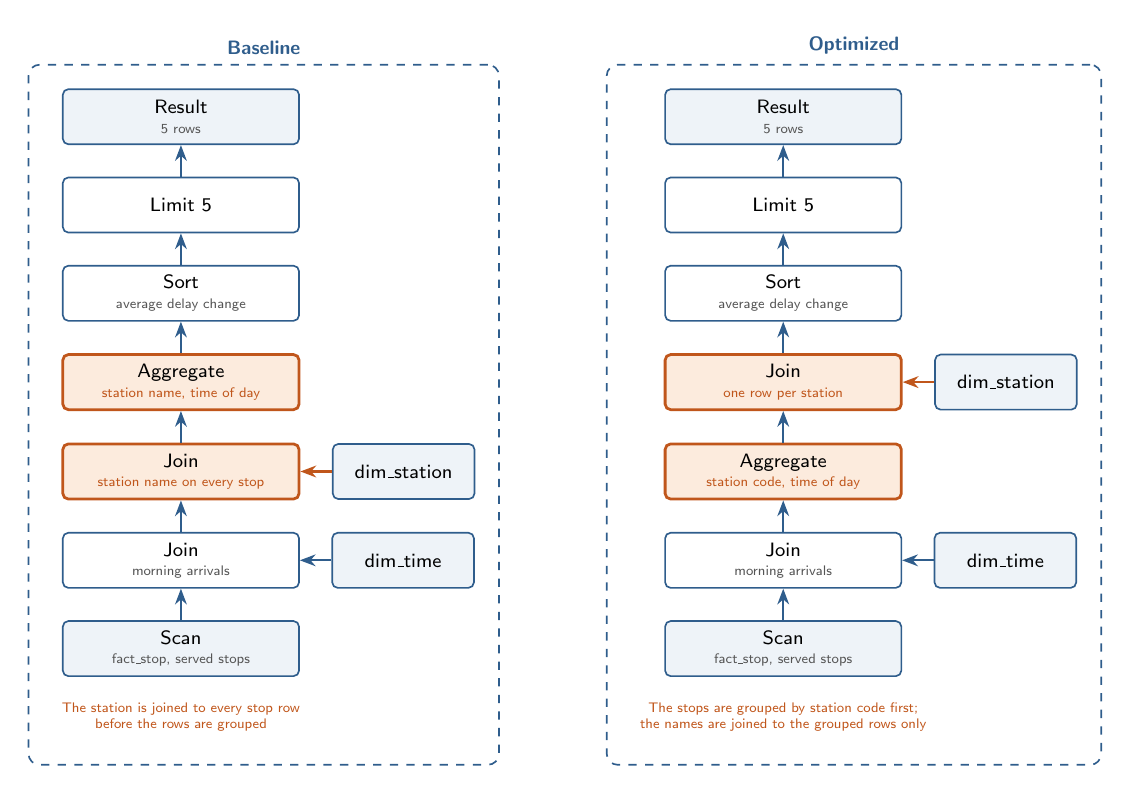
\begin{tikzpicture}

% ---------------- Baseline ----------------
\node[tbl] (bs) {Scan\\[-1pt]{\sub fact\_stop, served stops}};
\node[op, above=of bs] (bjt) {Join\\[-1pt]{\sub morning arrivals}};
\node[tbl, small, right=4mm of bjt] (btime) {dim\_time};
\node[op, hot, above=of bjt] (bjs) {Join\\[-1pt]{\hsub station name on every stop}};
\node[tbl, small, right=4mm of bjs] (bstat) {dim\_station};
\node[op, hot, above=of bjs] (ba) {Aggregate\\[-1pt]{\hsub station name, time of day}};
\node[op, above=of ba] (bo) {Sort\\[-1pt]{\sub average delay change}};
\node[op, above=of bo] (bl) {Limit 5};
\node[op, fill=groupfill, above=of bl] (br) {Result\\[-1pt]{\sub 5 rows}};

\draw[flow] (bs) -- (bjt);
\draw[flow] (btime) -- (bjt);
\draw[flow] (bjt) -- (bjs);
\draw[hotflow] (bstat) -- (bjs);
\draw[flow] (bjs) -- (ba);
\draw[flow] (ba) -- (bo);
\draw[flow] (bo) -- (bl);
\draw[flow] (bl) -- (br);

\node[callout, below=2mm of bs, align=center] (bnote)
    {The station is joined to every stop row\\before the rows are grouped};

\begin{scope}[on background layer]
  \node[panel, fit=(bs)(br)(bstat)(bnote)] (bp) {};
\end{scope}
\node[lbl, anchor=south] at (bp.north) {Baseline};

% ---------------- Optimized ----------------
\node[tbl, right=24mm of bs -| bstat.east, anchor=west] (os) {Scan\\[-1pt]{\sub fact\_stop, served stops}};
\node[op, above=of os] (ojt) {Join\\[-1pt]{\sub morning arrivals}};
\node[tbl, small, right=4mm of ojt] (otime) {dim\_time};
\node[op, hot, above=of ojt] (oa) {Aggregate\\[-1pt]{\hsub station code, time of day}};
\node[op, hot, above=of oa] (ojs) {Join\\[-1pt]{\hsub one row per station}};
\node[tbl, small, right=4mm of ojs] (ostat) {dim\_station};
\node[op, above=of ojs] (oo) {Sort\\[-1pt]{\sub average delay change}};
\node[op, above=of oo] (ol) {Limit 5};
\node[op, fill=groupfill, above=of ol] (or) {Result\\[-1pt]{\sub 5 rows}};

\draw[flow] (os) -- (ojt);
\draw[flow] (otime) -- (ojt);
\draw[flow] (ojt) -- (oa);
\draw[flow] (oa) -- (ojs);
\draw[hotflow] (ostat) -- (ojs);
\draw[flow] (ojs) -- (oo);
\draw[flow] (oo) -- (ol);
\draw[flow] (ol) -- (or);

\node[callout, below=2mm of os, align=center] (onote)
    {The stops are grouped by station code first;\\the names are joined to the grouped rows only};

\begin{scope}[on background layer]
  \node[panel, fit=(os)(or)(ostat)(onote)] (opp) {};
\end{scope}
\node[lbl, anchor=south] at (opp.north) {Optimized};

\end{tikzpicture}
\end{document}
